\documentclass[13, english]{report}
\usepackage[utf8]{inputenc}
\usepackage{graphicx}
\makeaother

\title{\textbf{Wind danger detector documentaion}}
\author{Marc Cervera rosell}
\date{January 2022}

\begin{document}
\pagestyle{empty}
\maketitle
\tableofcontents
\thispagestyle{empty}

\newpage

\chapter{Abstract}
\justify{This project, reads an input file with different values of wind gusts. The values are expressed in meters/second.\newline
In the other side, the program has a file with the danger level associated to the wind gusts.\newline
Once these two files are read, the neuronal network will have an entrance layer with the wind gusts and an output layer with the level of danger.\newline
When the user wants, he/she can enter an specific value to know what level of danger has that concrete wind gust.}

\pagenumbering{arabic}


\chapter{'.txt' files}
\section{inputs.txt}
\justify{This file has a few different values each of that represents a wind gust.\newline
The range values is from 0m/s to 200m/s. It has been considered that a wind gust greater than 200m/s is not relevant because a greater value is considered a tornado. Each value in the file is a float.}

\section{outputs.txt}
\justify{This is the complementary file of the above one. This file contents the danger level associated to his corresponding "brother" in "inputs.txt".\newline
Here, the meaning of "brother" is that each line \textit{i} of the "outputs.txt" file corresponds to the line \textit{i} of the "inputs.txt" file. Imagine that the "inputs.txt" file has a value of 31.25 on the line 12. Then the corresponding danger level in the "outputs.txt" file will be the value on line 12.}

\newpage

\chapter{Code}
\section{\textit{read data file} method}
\justify{This first method, stores the value of each line of the file inside a list that will be returned at the end.\newline
The fist step is to open in \textit{reading} mode, the file given as the only mandatory parameter of the method. Secondly, for each line in the file (data + newline character), the algorithm, stores in a variable the splited line by the non mandatory parameter. This last operation, gives us a tuple seen as:\newline
\begin{table}[h]
    \centering
    \begin{tabular}{|c|c|}
        \hline
         \textit{"Value"} & \textit{"newline character"}\\ \hline
    \end{tabular}
    \caption{Tuple}
    \label{tab:my_label}
\end{table}
\newline Finally, before closing the read file and returning the data list, the algorithm appends to the data list only the float number.\newline
Once the two files are read, we've to convert to the corresponding type the values because at this time, the lists that contents the inputs and the outputs, have \textit{String} and not \textit{float} or \textit{int}. Therefore, the algorithm converts them with a loop and making a cast for each position of the list.\newline
Outside of the method, the two lists are converted to arrays with the function \textit{array} from \textit{numpy}.}

\section{Neuronal network}
\subsection{Layers and model creation}
\justify{This program has an input neuron, two hidden layers and an output layer.\newline
The hidden ones are \textit{Dense} layers with 10 neurons each one. To create this two hidden layers the \textit{Tensorflow} library has been used.\newline
Finally, the algorithm creates the model as a Sequential model and it adds all the layers that it has created.}
\subsection{Compiling}
\justify{To compile the model, the programmer (myself) has to choose an optimizer and a loss function. In this case the choosen optimizer is \textit{Adam} and the choosen loss function is \textit{mean squared error}.\newline
The optimizer, allows the layer to adjust biases and weights efficiently for it to learn and the number tells the optimizer how much to adjust the weights and the biases.\newline
The choosen loss function, considers that a small amount of large errors is worse than a large amount of small errors.}

\subsection{Training the model}
\justify{To train the model the algorithm uses the \textit{fit} method. Two mandatory parameters are given to this method and two non mandatory more:\newline 
\begin{center}
    \textit{model.fit(inputs, outputs, epochs, verbose)}\newline
\end{center}
As it has been said, the two first parameters are mandatory, the other two not.}

\subsection{Printing the loss function graphic}
\justify{Using the \textit{matplotlib.pyplot} import, the program shows the graphic of the loss function.\newline
The loss function tells the programmers/users how bad are the results of the network in each epoch. Hence, the more epochs are completed the fewer errors there are.\newline
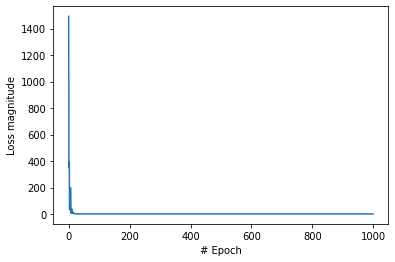
\includegraphics[]{download.png}}

\chapter{Playing with predictions}
\justify{Finally, once all the work is done, a random user can use this program to obtain predictions.\newline
To make a prediction, the user only has to change the parameter of the \textit{model.predict} method and run the program. The danger level of the introduced wind gust will be shown.}

\end{document}
